
A palavra \emph{Sistema} tem origem no grego \emph{synístanai} e de acordo com \cite{gramaticaNET} significa "fazer funcionar junto" e uma aplicação precursora do controle é apresentada por Ctesibius de Alexandria ( \cite{encyclopediaBritannica} ) onde um conjunto de reservatórios de água com furo na parte inferior geravam por gotejamento uma marcação do tempo, porém a água do reservatório precisa estar em um nível constante, pois o intervalo de gotejamento é afetado diretamente pela quantidade de água, assim foi criado por Ctesibius um sistema semelhante as boias dos reservatórios atuais para manter o nível de água no reservatório sempre constante.

A modificação do comportamento de um sistema, de forma controlada garantindo uma maior eficiência é o objetivo do controle de sistemas. 

A principal tarefa de um engenheiro, segundo \cite{dorf2011modern} "é o processo de concepção ou invenção de formas, partes e detalhes de um sistema para alcançar um propósito específico", processo este que soma a grande capacidade de análise e a criatividade para atender as demandas da função, como é o caso de projeto em engenharia no segmento de Sistemas de controle, cujo objetivo é obter configuração, especificações e identificação de processos para atender uma necessidade real. Norman S. Nise traz uma concepção semelhante onde "Um sistema de controle consiste em subsistemas e processos(ou plantas) construídos com o objetivo de se obter uma saída desejada com desempenho desejado para uma entrada específica fornecida".

Os sistemas de controle atuam basicamente gerando respostas específicas para estímulos específicos de forma controlada e automática trazendo vantagens nas aplicações de diversas áreas como movimentação de grandes equipamentos com precisão, aplicação em locais remotos ou perigosos, compensação de perturbações, manipulação de dados convenientes etc.



%%%%%%%%%%%%%%%%%%%%%%%%%%%%%%%%%%%%%%%%%%%%%%%%%%%%%%%%%%%%
\section{Diagrama de Blocos}
%%%%%%%%%%%%%%%%%%%%%%%%%%%%%%%%%%%%%%%%%%%%%%%%%%%%%%%%%%%%

Os sistemas de controle são geralmente representados através de diagramas de blocos ou fluxo de sinais, como na Figura \ref{fig:processo} convenientes ao seu desenvolvimento e análise. É composta por uma caixa representando o sistema a ser controlado, setas no sentido da caixa representando as entradas do processo e setas no sentido para fora da caixa para indicar a saída do sistema.

Em um sistema real podem haver muitas variáveis de entrada e de saída, mas a abordagem clássica de controle isola apenas uma das variáveis de entrada e uma de saída, ficando o sistema conhecido pela sigla em inglês SISO (\emph{Single In Single Out} - Única Entrada e Única Saída).

\begin{figure}[!htb]
\centering
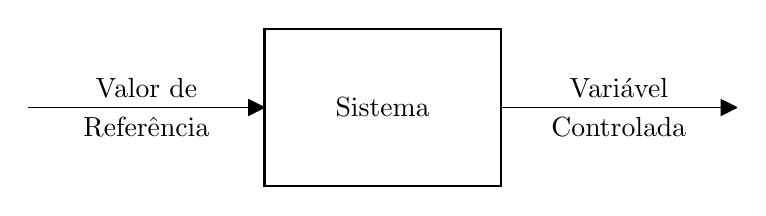
\begin{tikzpicture}[scale=1]
%\draw [lightgray](0,0) grid (9,2);
\draw (0,1) -- (3,1);
\draw [black, thick](3,0) rectangle (6, 2) ; 
\draw (6,1) -- (9,1);

\draw [fill](3,1) -- (2.8, 1.1) -- (2.8,0.9) -- (3,1);
\draw [fill](9,1) -- (8.8, 1.1) -- (8.8,0.9) -- (9,1);

\node at (4.5, 1){Sistema};
\node [above] at (1.5,1){Valor de};
\node [below] at (1.5,1){Referência};
\node [above] at (7.5,1){Variável};
\node [below] at (7.5,1){Controlada};
\end{tikzpicture}
\caption{ Diagrama de blocos de sistema de controle}
\label{fig:processo}
\end{figure}


O diagrama de blocos mostrado na Figura \ref{fig:processo} é uma simplificação ao máximo de um sistema de controle, contém apenas o bloco representando o sistema, uma entrada, para o valor de referência, e uma saída com o valor da variável controlada. A Figura \ref{fig:malhaAberta}, divide os bloco do sistema em dois: controlador e planta. Neste caso, um sistema de controle em malha aberta, ou seja, não há uma reinserção do sinal de saída à entrada, chamada de realimentação ou retroalimentação. Assim, a entrada possui o valor de resposta desejada, que alimenta o processo e a saída apresenta a resposta real, porém nada garante que a resposta real está coerente ao valor de entrada.

\begin{figure}[!htb]
\centering
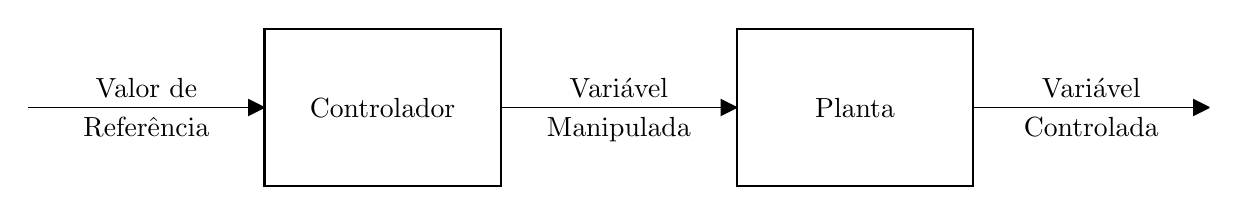
\begin{tikzpicture}[scale=1]
%\draw [lightgray](0,0) grid (15,2);
\draw (0,1) -- (3,1);
\draw [black, thick](3,0) rectangle (6, 2) ; 
\draw (6,1) -- (9,1);
\draw [black, thick](9,0) rectangle (12, 2) ; 
\draw (12,1) -- (15,1);

\draw [fill]( 3,1) -- ( 2.8, 1.1) -- ( 2.8,0.9) -- ( 3,1);
\draw [fill]( 9,1) -- ( 8.8, 1.1) -- ( 8.8,0.9) -- ( 9,1);
\draw [fill](15,1) -- (14.8, 1.1) -- (14.8,0.9) -- (15,1);

\node at ( 4.5, 1){Controlador};
\node at (10.5, 1){Planta};
\node [above] at ( 1.5,1){Valor de};
\node [below] at ( 1.5,1){Referência};
\node [above] at ( 7.5,1){Variável};
\node [below] at ( 7.5,1){Manipulada};
\node [above] at (13.5,1){Variável};
\node [below] at (13.5,1){Controlada};
\end{tikzpicture}
\caption{ Diagrama de blocos de sistema de controle em malha aberta}
\label{fig:malhaAberta}
\end{figure}

O diagrama da Figura \ref{fig:malhaFechada} apresenta realimentação, ou seja, uma amostra da resposta real é lida por um elemento sensor e é reinserida à entrada da malha, aonde é realizada a comparação entre resposta real e desejada, a diferença entre ambos os valores é chamado de Erro do Sistema e é baseado nesse valor que o controlador tem condições de efetuar as devidas correções, geralmente, afim de manter o sistema estável no valor de resposta desejada.

\begin{figure}[!htb]
\centering
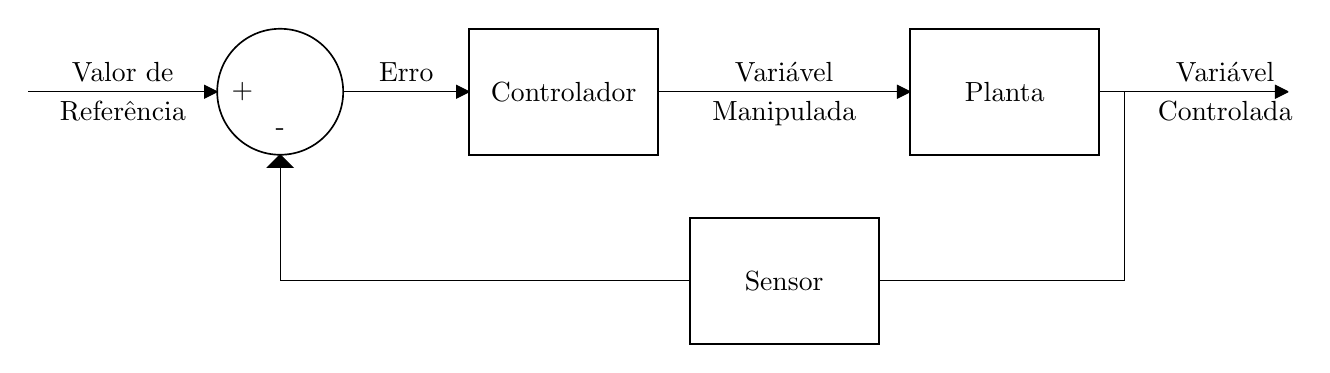
\begin{tikzpicture}[scale=0.8]
%\draw [lightgray](-3,0) grid (17, 2);
%\draw [lightgray](-3,0) grid (17,-3);
%\draw [semithick,red] (0,0) circle (0.1);

\draw (-3,1) -- (0,1);
\draw [fill]( 0,1) -- (-0.2, 1.1) -- ( -0.2,0.9) -- (0,1);
\draw [semithick,black] (1,1) circle (1.0); % Somador
\draw (2.0,1) -- (4,1);
\draw [fill]( 4,1) -- ( 3.8, 1.1) -- ( 3.8,0.9) -- ( 4,1);
\draw [black, thick](4,0) rectangle (7, 2) ; % Controlador 
\draw (7,1) -- (11,1);
\draw [fill]( 11,1) -- (10.8, 1.1) -- (10.8,0.9) -- (11,1);
\draw [black, thick](11,0) rectangle (14, 2) ; % Planta
\draw (14,1) -- (17,1);
\draw [fill](17,1) -- (16.8, 1.1) -- (16.8,0.9) -- (17,1);

\draw [black, thick](7.5,-1) rectangle (10.5, -3) ; % Sensor
\draw (14.4, 1) -- (14.4, -2) -- (10.5,-2);
\draw ( 7.5,-2) -- ( 1, -2) -- (1,0);
\draw [fill](1,0) -- (1.2,-0.2) -- (0.8,-0.2) -- (1,0);

\node [above] at (-1.5,1){Valor de};
\node [below] at (-1.5,1){Referência};
\node at (0.4,1){+};
\node at (1,0.4){-};
\node [above] at (3.0,1){Erro};
\node at ( 5.5, 1){Controlador};
\node [above] at (9.0,1){Variável};
\node [below] at (9.0,1){Manipulada};
\node at (12.5, 1){Planta};
\node [above] at (16.0,1){Variável};
\node [below] at (16.0,1){Controlada};
\node at ( 9.0,-2){Sensor};

\end{tikzpicture}
\caption{ Diagrama em blocos de sistema de controle em malha fechada}
\label{fig:malhaFechada}
\end{figure}


Como notação para os elementos do diagrama de blocos, são adotadas letras para representar matematicamente as relações entre as grandezas conforme Figura  \ref{fig:malhaFechadaLetras}


\begin{figure}[!htb]
\centering
\begin{tikzpicture}[scale=0.8]
%\draw [lightgray](-3,0) grid (17, 2);
%\draw [lightgray](-3,0) grid (17,-3);
%\draw [semithick,red] (0,0) circle (0.1);

\draw (-3,1) -- (0,1);
\draw [fill]( 0,1) -- (-0.2, 1.1) -- ( -0.2,0.9) -- (0,1);
\draw [semithick,black] (1,1) circle (1.0); % Somador
\draw (2.0,1) -- (4,1);
\draw [fill]( 4,1) -- ( 3.8, 1.1) -- ( 3.8,0.9) -- ( 4,1);
\draw [black, thick](4,0) rectangle (7, 2) ; % Controlador 
\draw (7,1) -- (11,1);
\draw [fill]( 11,1) -- (10.8, 1.1) -- (10.8,0.9) -- (11,1);
\draw [black, thick](11,0) rectangle (14, 2) ; % Planta
\draw (14,1) -- (17,1);
\draw [fill](17,1) -- (16.8, 1.1) -- (16.8,0.9) -- (17,1);

\draw [black, thick](7.5,-1) rectangle (10.5, -3) ; % Sensor
\draw (14.4, 1) -- (14.4, -2) -- (10.5,-2);
\draw ( 7.5,-2) -- ( 1, -2) -- (1,0);
\draw [fill](1,0) -- (1.2,-0.2) -- (0.8,-0.2) -- (1,0);

\node [above] at (-1.5,1){r(t)};
\node at (0.4,1){+};
\node at (1,0.4){-};
\node [above] at (3.0,1){e(t)};
\node at ( 5.5, 1){f(t)};
\node [above] at (9.0,1){u(t)};
\node at (12.5, 1){g(t)};
\node [above] at (16.0,1){c(t)};
\node at ( 9.0,-2){h(t)};

\end{tikzpicture}
\caption{ Diagrama em blocos de sistema de controle em malha fechada utilizando notação matemática}
\label{fig:malhaFechadaLetras}
\end{figure}



%%%%%%%%%%%%%%%%%%%%%%%%%%%%%%%%%%%%%%%%%%%%%%%%%%%%%%%%%%%%
\section{Controle Clássico}
%%%%%%%%%%%%%%%%%%%%%%%%%%%%%%%%%%%%%%%%%%%%%%%%%%%%%%%%%%%%

Os sistemas de controle clássicos possuem a predileção por tratar sistemas monovariáveis, lineares e invariantes no tempo, mas esta não é a condição mais provável para um sistema físico. Ao longo do tempo foram desenvolvidas ferramentas, como a Transformada de Laplace, para contornar algumas dificuldades inerentes ao equacionamento dos modelos matemáticos e também métodos como o dos lugares das raízes ou resposta de frequência.

Os sistemas de controle modernos possuem o índice de desempenho em termos de variáveis de estado, e possuem técnicas para tratar sistemas multivariáveis, não lineares e variantes no tempo.

A forma prática de trabalhar com sistemas de controle clássicos é através de modelos matemáticos para descrever a dinâmica dos sistemas a partir das leis físicas que regem seus comportamento e desempenho.
As variáveis dos sistemas articulam-se dinamicamente e são expressas matematicamente utilizando, geralmente, equações diferencias, e podem ser relações lineares ou não lineares. Para sistemas não lineares é habitual que seja feita a linearização do sistema, ou de uma região que se queira controlar, utilizando como ferramenta a Série de Taylor. 

Outra ferramenta extremamente importante é a Transformada de Laplace que converte uma equação diferencial no domínio do tempo em uma equação algébrica no domínio da frequência, facilitando a manipulação matemática na utilização dos métodos de controle. 

A relação das variáveis de saída com a de entrada do sistema, é denominada de Função de Transferência(FT) e apresenta as características dinâmicas do sistema.



%%%%%%%%%%%%%%%%%%%%%%%%%%%%%%%%%%%%%%%%%%%%%%%%%%%%%%%%%%%
\subsection{Modelagem matemática}
%%%%%%%%%%%%%%%%%%%%%%%%%%%%%%%%%%%%%%%%%%%%%%%%%%%%%%%%%%%

A maioria dos sitemas físicos pode ser modelado matematicamente através de equações diferenciais parciais e é comum que os sistemas apresentem comportamento exponencial, e também apresentam não linearidades, que dependendo da aplicação, podem ser aproximadas em regiões específicas de operação e as equações sofrem transformadas para simplificar a manipulação e resolução dos problemas encontrados nos diversos sistemas assim como o apresentado neste estudo.


%%%%%%%%%%%%%%%%%%%%%%%%%%%%%%%%%%%%%%%%%%%%%%%%%%%%%%%%%%%
\subsection{Sistema Linear}
%%%%%%%%%%%%%%%%%%%%%%%%%%%%%%%%%%%%%%%%%%%%%%%%%%%%%%%%%%%

Quase que a totalidade dos processos naturais apresentam aspectos não lineares, porém a técnica de controle clássico trabalha apenas com sistemas lineares, assim exitem duas opções para trabalhar com sistemas não lineares: mudar o método de controle para uma ténica não convencional ou linearizar em torno de um ponto de operação. A linearização é o processo de encontrar um modelo linear que atenda bem a aproximação do modelo não linear em questão.

Lyapunov ??? provou que em uma região próxima ao ponto de operação um sistema não linear pode ser estável.

Dado um sistema \emph{S(t)} para uma entrada $u(t) = u_1(t)$ tem-se uma saída $y(t) = y_1(t)$ e para uma entrada $u(t) = u_2(t)$ tem-se uma saída $y(t) = y_2(t)$.

\begin{figure}[!htb]
\centering
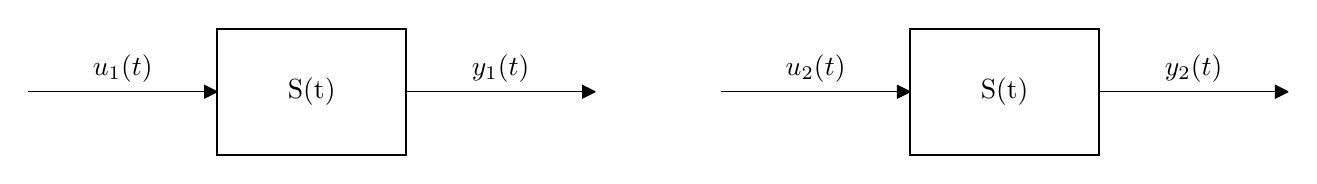
\begin{tikzpicture}[scale=0.8]
%\draw [lightgray](0,0) grid (20, 2);

\draw (0,1) -- (3,1);
\draw [fill]( 3,1) -- ( 2.8, 1.1) -- ( 2.8,0.9) -- ( 3,1);
\draw [black, thick](3,0) rectangle (6, 2) ; % S1 
\draw (6,1) -- (9,1);
\draw [fill]( 9,1) -- (8.8, 1.1) -- (8.8,0.9) -- (9,1);

\draw (11,1) -- (14,1);
\draw [fill]( 14,1) -- ( 13.8, 1.1) -- ( 13.8,0.9) -- ( 14,1);
\draw [black, thick](14,0) rectangle (17, 2) ; % S2
\draw (17,1) -- (20,1);
\draw [fill]( 20,1) -- (19.8, 1.1) -- (19.8,0.9) -- (20,1);


\node [above] at (1.5,1){$u_1(t)$};
\node at ( 4.5, 1){S(t)};
\node [above] at (7.5,1){$y_1(t)$};

\node [above] at (12.5,1){$u_2(t)$};
\node at ( 15.5, 1){S(t)};
\node [above] at (18.5,1){$y_2(t)$};

\end{tikzpicture}
\caption{ Sistema simples}
\label{fig:sistemaSimples}
\end{figure}

Assim para a região linear próxima ao ponto de operação, uma combinação linear na entrada $u(t) = \alpha u_1(t) + \beta u_2(t)$ produz $y(t) = \alpha y_1(t) + \beta y_2(t), \forall \alpha ,  \beta \in \Re $, que é o princípio da superposição ilustrado na Figura \ref{fig:principioSuperposicao}.


\begin{figure}[!htb]
\centering
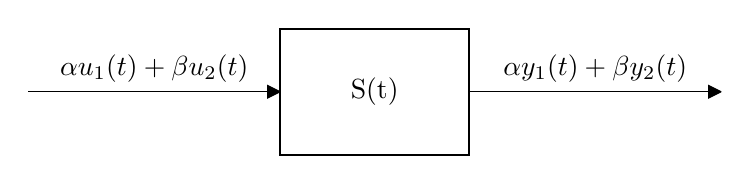
\begin{tikzpicture}[scale=0.8]
%\draw [lightgray](0,0) grid (11, 2);

\draw (0,1) -- (4,1);
\draw [fill]( 4,1) -- ( 3.8, 1.1) -- ( 3.8,0.9) -- ( 4,1);
\draw [black, thick](4,0) rectangle (7, 2) ; % S1 
\draw (7,1) -- (11,1);
\draw [fill]( 11,1) -- (10.8, 1.1) -- (10.8,0.9) -- (11,1);

\node [above] at (2,1){$\alpha u_1(t) + \beta u_2(t)$};
\node at ( 5.5, 1){S(t)};
\node [above] at (9,1){$\alpha y_1(t) + \beta y_2(t)$};

\end{tikzpicture}
\caption{ Princípio da Superposição}
\label{fig:principioSuperposicao}
\end{figure}



%%%%%%%%%%%%%%%%%%%%%%%%%%%%%%%%%%%%%%%%%%%%%%%%%%%%%%%%%%%
\subsubsection{Linearização}
%%%%%%%%%%%%%%%%%%%%%%%%%%%%%%%%%%%%%%%%%%%%%%%%%%%%%%%%%%%

Para o processo de linearização de um sinal, uma forma comumente utilizada é através da Série de Taylor, onde dado um plano cartesiano e uma função \emph{f} com um ponto qualquer com coordenadas \emph{x} e \emph{y} com pequenas variações $\overline{x}$ e $\overline{y}$, temos que:

\begin{center}
\begin{equation}
y = \overline{y} + 
\frac{df}{dx} \left| \frac{ }{ } _{\overline{x}} \right. \, (x - \overline{x}) + 
\frac{1}{2!} \frac{d²f}{dx²} \left| \frac{ }{ } _{\overline{x}} \right. \, (x - \overline{x})² +
\frac{1}{3!} \frac{d³f}{dx³} \left| \frac{ }{ } _{\overline{x}} \right. \, (x - \overline{x})³ + ...
\label{eqn:SerieTaylor}
\end{equation}
\end{center}

A Série de Taylor é truncada após o segundo membro da somatória, pois $(x - \overline{x}^n )$ é cada vez menor na medida em que o expoente aumenta, fazendo com que tal parcela da somatória tenda a zero, assim despreza-se tais termos e tem-se:

\begin{center}
\begin{equation}
y = \overline{y} + 
\frac{df}{dx} \left| \frac{ }{ } _{\overline{x}} \right. \, (x - \overline{x})
\label{eqn:SerieTaylorTruncada}
\end{equation}
\end{center}



%%%%%%%%%%%%%%%%%%%%%%%%%%%%%%%%%%%%%%%%%%%%%%%%%%%%%%%%%%%
\subsection{Transformada de Laplace}
%%%%%%%%%%%%%%%%%%%%%%%%%%%%%%%%%%%%%%%%%%%%%%%%%%%%%%%%%%%
 
A Transformada de Laplace é utilizada em controle como uma ferramenta matemática para facilitar a solução de equações diferenciais lineares, utilizando uma variável complexa \emph{s}, operações como derivação e integração podem ser substituidas por operações algébricas no plano complexo, domínio da frequência, e após a resolução realiza-se a Transformada Inversa de Laplace para retornar a solução para o domínio do tempo.

A definição e sua dedução de forma rigorosa podem ser encontradas em \cite{Ogata} e não será discutida neste trabalho, mas vale aqui apresentar apenas a sua definição e uma parte da tabela de conversão.

A Transformada de Laplace é definida como:

\begin{equation}
\mathscr{L}\{f(t)\} = F(s) = \int_{0}^{\infty} f(t) e^{-st} dt
\label{eq:transfLaplace}
\end{equation} 

Onde:

\setlength{\parindent}{2cm}
$\mathscr{L}$ : Operador da Transformada de Laplace 

$f(t)$ : função da variável $t$ tal que $f(t) = 0$ para $t < 0$ 

$F(s)$ : Transformada de Laplace de $f(t)$

$s$ : variável complexa
\\

\setlength{\parindent}{0cm}
A Transformada Inversa de Laplace é definida como:

\begin{equation}
\mathscr{L}^{-1} \{F(s)\} =  \frac{1}{2 \pi j} \int_{c-j\infty}^{c+j\infty}F(s) e^{st} ds  \text{ , para } t > 0
\label{eq:transfInvLaplace}
\end{equation}

Onde:

\setlength{\parindent}{2cm}
$\mathscr{L}^{-1}$ : Operador da Transformada Inversa de Laplace

$c$ : Número real constante, abscissa da convergência.

\setlength{\parindent}{1cm}

Dificilmente a Transformada Inversa de Laplace é utilizada, podendo ser utilizado o método de frações parciais ou a tabela de conversão.

A Tabela \ref{tab:Laplace} mostra alguns pares de Transformadas de Laplace, e uma tabela mais completa pode ser encontrada no Capítulo 2 de \cite{Ogata}. 

\begin{table}[h]
\centering
\caption{Pares de Transformadas de Laplace}
\label{tab:Laplace}
\begin{tabular}{c|c}
\hline
$f(t)$ & $F(s)$ \\
\hline
\hline
Impulso unitário $\delta(t)$ 		& $1$ 			\\ \hline
Degrau unitário $1(t)$ 			& $\frac{1}{s}$		\\ \hline
$t$ 					& $\frac{1}{s^2}$ 	\\ \hline
$\frac{t^{n-1}}{(n-1)!} (n=1,2,3,...)$ 	& $\frac{1}{s^n}$ 	\\ \hline
$t^n (n=1,2,3,...)$ 			& $\frac{n!}{s^{n+1}}$ 	\\ \hline
$e^{-at}$ 				& $\frac{1}{s+a}$ 	\\ \hline
$t^n e^{-at} (n=1,2,3,...)$ 		& $\frac{n!}{(s+a)^{n+1}}$ \\\hline
$\frac{1}{a} (1-e^{-at})$ 		& $\frac{1}{s(s+a)}$ 	\\ \hline
$\frac{1}{b-a}(e^{-at}-e^{-bt})$ 	& $\frac{1}{(s+a)(s+b)}$ \\ \hline
\end{tabular}
\end{table}






%%%%%%%%%%%%%%%%%%%%%%%%%%%%%%%%%%%%%%%%%%%%%%%%%%%%%%%%%%%
\section{Ação de Controle}
%%%%%%%%%%%%%%%%%%%%%%%%%%%%%%%%%%%%%%%%%%%%%%%%%%%%%%%%%%%

As ações de controle, são tomadas afim de atender as especificações e os requisitos de desempenho de cada sistema. Assim, utilizando o sistema descrito em detalhes no Capítulo 3 Sistema Eletrônico, é mostrado o resultado da implementação das principais ações de controle para uma implementação em malha aberta e em malha fechada.

\subsection{ Malha Aberta }

O controle em malha aberta é o sistema mais simples de ser implementado, não possui realimentação, ou seja, o controlador não possui uma indicação da variável controlada, não sendo possível a sua correção caso haja alguma interferência, oscilação, ruído, ou mesmo que o sistema não apresente baixo rendimento.

\begin{figure}[!htb]
\centering
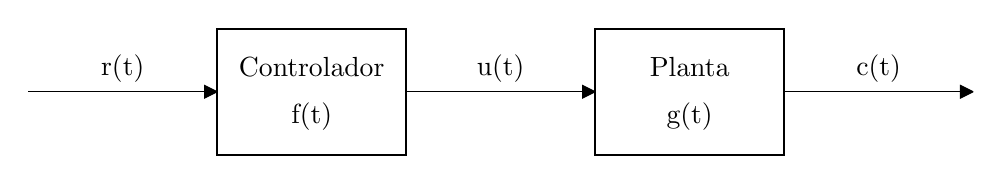
\begin{tikzpicture}[scale=0.8]
%\draw [lightgray](0,0) grid (15,2);
\draw (0,1) -- (3,1);
\draw [black, thick](3,0) rectangle (6, 2) ; 
\draw (6,1) -- (9,1);
\draw [black, thick](9,0) rectangle (12, 2) ; 
\draw (12,1) -- (15,1);

\draw [fill]( 3,1) -- ( 2.8, 1.1) -- ( 2.8,0.9) -- ( 3,1);
\draw [fill]( 9,1) -- ( 8.8, 1.1) -- ( 8.8,0.9) -- ( 9,1);
\draw [fill](15,1) -- (14.8, 1.1) -- (14.8,0.9) -- (15,1);

\node at ( 4.5, 1.4){Controlador};
\node at ( 4.5, 0.6){f(t)};
\node at (10.5, 1.4){Planta};
\node at (10.5, 0.6){g(t)};
\node [above] at ( 1.5,1){r(t)};
\node [above] at ( 7.5,1){u(t)};
\node [above] at (13.5,1){c(t)};
\end{tikzpicture}
\caption{ Sistema de controle em malha aberta}
\label{fig:AcaoMalhaAberta}
\end{figure}

O sistema físico aqui estudado possui comportamento exponencial que pode ser descrito pela equação \ref{eq:ftSistOrdem1}. 




\begin{equation}
	 \frac{d c(t)}{dt} + c(t) = r(t) \rightarrow  \mathscr{L} \to \frac{C(s)}{R(s)} = \frac{K}{s + a} 
\label{eq:ftSistOrdem1}
\end{equation}

%\begin{equation}
%\therefore \frac{C(s)}{R(s)} = \frac{k}{s+a}
%\label{eq:ftSistOrdem1}
%\end{equation}

Onde:

\setlength{\parindent}{2cm}

$t$ : tempo,$ r(t) = 0$ , para t $<$ 0;

$\mathscr{L}$ : Operador de Laplace;

$c(t)$ : Variável controlada no domínio do tempo;

$C(s)$ : Variável controlada no domínio da frequência;

$r(t)$ : Valor de referência (\emph{setpoint}) no domínio do tempo;

$R(s)$ : Valor de referência (\emph{setpoint}) no domínio da frequência.

$K$ : Constantede proporcionalidade;

$s$ : Variável complexa de Laplace;

$a$ : Polo da função.
\setlength{\parindent}{1cm}

Sendo assim, para um estímulo de entrada do tipo \textbf{degrau}, com amplitude \textbf{A}, temos $ R(s) = \frac{A}{s}$ e aplicando a Transformada Inversa de Laplace:

\begin{equation}
C(s) = \frac{K}{s+a} \frac{A}{s} \rightarrow \mathscr{L}^{-1} \to c(t) = \frac{K A}{a} (1 - e^{-at})
\label{eq:degrauA}
\end{equation}

A Figura \ref{fig:degrauA} mostra um sinal do tipo degrau com amplitude \textbf{A} aplicado ao sistema de teste, que responde conforme um conforme um sistema de primeira ordem como mostrado na Figura \ref{fig:cRegime}. A partir de um determinado instante de tempo, entra em regime constante ($c_{reg}$), alcançando o valor de referência dado pelo degrau de amplitude A. Assim quando $ t \rightarrow \infty $  então $ c_{reg} \rightarrow A $:


\begin{figure}
\centering
\subfloat[Sinal de entrada tipo degrau com amplitude A]{\label{fig:degrauA}
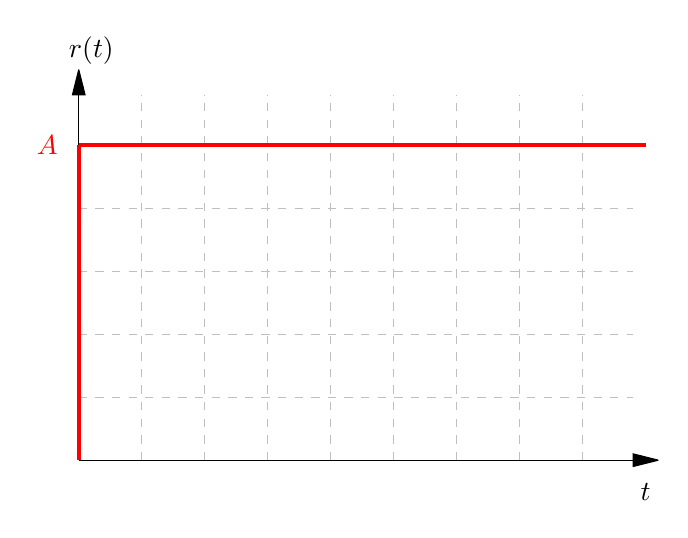
\begin{tikzpicture}[scale=0.8]
\draw [lightgray, dashed](0,0) grid (8.8,5.8);
\draw [->] (0,0) -- (9,0);
\draw [fill] (0,6.2) -- (-0.1, 5.8) -- (0.1,5.8) -- (0,6.2);
\draw [->] (0,0) -- (0,6);
\draw [fill] (9.2,0) -- (8.8,0.1) -- (8.8,-0.1)--(9.2,0.0);
\node at (9.0,-0.5) {$t$};
\node at (0.2,6.5) {$r(t)$};
\draw [red, ultra thick] (0.0,5.0) -- (9.0,5.0);
\draw [red, ultra thick] (0.0,0.0) -- (0.0,5.0);
\node at (-0.5,5.0)[red]{$A$};
\end{tikzpicture} }
\subfloat[Resposta transitória e regime de acomodação]{\label{fig:cRegime}
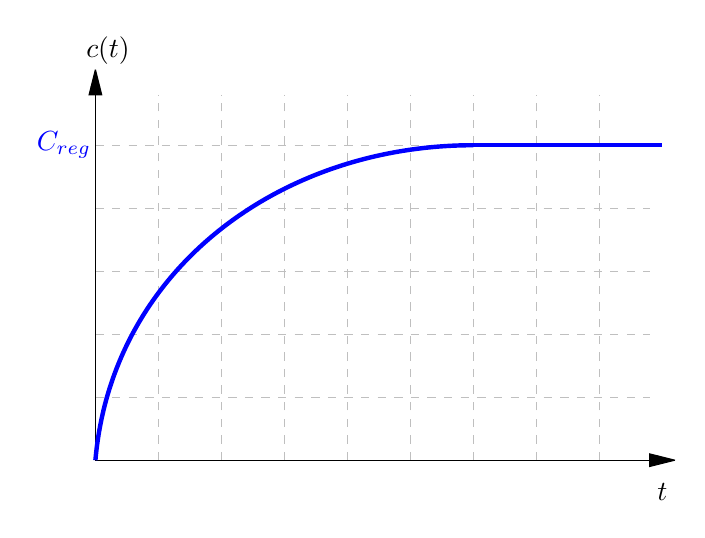
\begin{tikzpicture}[scale=0.8]
\draw [lightgray, dashed](0,0) grid (8.8,5.8);
\draw [->] (0,0) -- (9,0);
\draw [fill] (0,6.2) -- (-0.1, 5.8) -- (0.1,5.8) -- (0,6.2);
\draw [->] (0,0) -- (0,6);
\draw [fill] (9.2,0) -- (8.8,0.1) -- (8.8,-0.1)--(9.2,0.0);
\node at (9.0,-0.5) {$t$};
\node at (0.2,6.5) {$c(t)$};
\node at (-0.5,5.0)[blue]{$C_{reg}$};
\draw [blue, ultra thick] (0,0) to [out=85, in=180] (6,5);
\draw [blue, ultra thick] (6,5) -- (9,5);
\end{tikzpicture}}
\caption{Sistema de Primeira Ordem}
\label{fig:sistPrimeiraOrdem}
\end{figure}

%\begin{equation}
%c_{reg} = \lim_{t \rightarrow \infty} \frac{KA}{a}(1-e^{-at}) = \frac{KA}{a}
%\label{eq:cregime}
%\end{equation}

Aplicando o Teorema do Valor Final pode-se ver que o \emph{$c_{reg}$} estabiliza em um valor constante como mostrado pela Equação \ref{eq:teoremaValorFinal}:

\begin{equation}
C_{reg} = \lim_{s \rightarrow 0} sC(s) = \lim_{s \rightarrow 0} s\ \frac{K}{s+a}\frac{A}{s} = \frac{KA}{a}
\label{eq:teoremaValorFinal}
\end{equation}

Matematicamente, quanto maior o valor de \emph{t} na Equação \ref{eq:degrauA}, o resultado de sua exponenencial tende a zero, levando a um resultado que depende apenas das constantes, como mostrado na Equação \ref{eq:teoremaValorFinal}. 

Tomando $t= \frac{1}{a} = a^{-1} = \tau$ para gerar um valor conhecido em $e^{-at}$, da Equação \ref{eq:degrauA} temos:


\begin{equation}
c(a^-1) = \frac{KA}{a}(1-e^{-(a.a^{-1})}) = \frac{KA}{a}(1-e^{-1}) = \frac{KA}{a}.0,63 = 0,63 . C_{reg}
\end{equation}

A Figura \ref{fig:constTempo} mostra a constante de tempo $\tau$, que é atingida quando o sistema alcança 63\% do seu valor de regime. Como sabemos que $\tau = \frac{1}{a}$, então o polo do sistema, que leva o denominador da Equação \ref{eq:degrauA} a zero, é:

\begin{equation}
a = \frac{1}{\tau}
\end{equation}



\begin{figure}
\centering
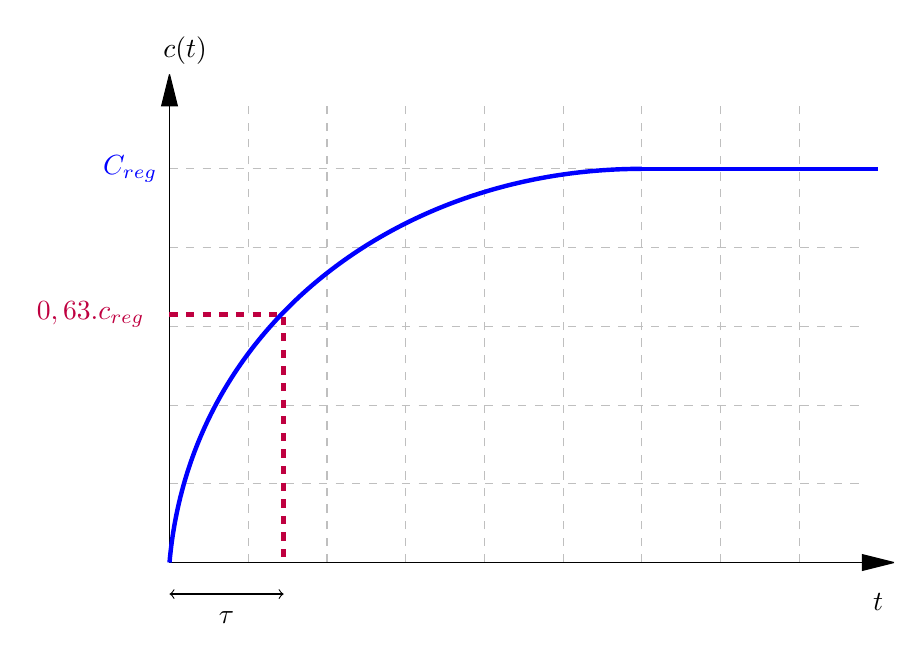
\begin{tikzpicture}[scale=1.0]
\draw [lightgray, dashed](0,0) grid (8.8,5.8);

\draw [->] (0,0) -- (9,0);
\draw [fill] (0,6.2) -- (-0.1, 5.8) -- (0.1,5.8) -- (0,6.2);
\draw [->] (0,0) -- (0,6);
\draw [fill] (9.2,0) -- (8.8,0.1) -- (8.8,-0.1)--(9.2,0.0);

\node at (9.0,-0.5) {$t$};
\node at (0.2,6.5) {$c(t)$};

\node at (-0.5,5.0)[blue]{$C_{reg}$};
\node at (-1,5.0*0.63)[purple]{$0,63.c_{reg}$};
\draw [purple, ultra thick, dashed] (0.0,5.0*0.63) -- (1.45,5.0*0.63)
						   -- (1.45,0.0);
\draw [blue, ultra thick] (0,0) to [out=85, in=180] (6,5);
\draw [blue, ultra thick] (6,5) -- (9,5);

\draw [<->] (0.0,-0.4) -- (1.45,-0.4); 
\node at (1.45/2,-0.7){$\tau$};

\end{tikzpicture}
\caption{Constante de tempo}
\label{fig:constTempo}
\end{figure}

Portanto:

\begin{equation}
K = \frac{ac_{reg}}{A}
\label{eq:calcK}
\end{equation}

%\begin{tikzpicture}
%\begin{axis}
%\addplot[title=Gráfico de uma função, 
%	xlabel = {$x$}, ylabel={$y$},
% 	red!70!blue, very thick, samples=200,
%	domain=-3:3]{x/(x^4-3*x^2+4)};
%\end{axis}
%\end{tikzpicture}







A Figura \ref{fig:AcaoMalhaAberta} mostra um sinal do tipo degrau aplicado como referência no valor de \emph{25 rps}, a curva de comportamento real medida empiricamente e a curva aproximada calculada pelo método determinístico como segue:

\begin{figure}[!htb]
\center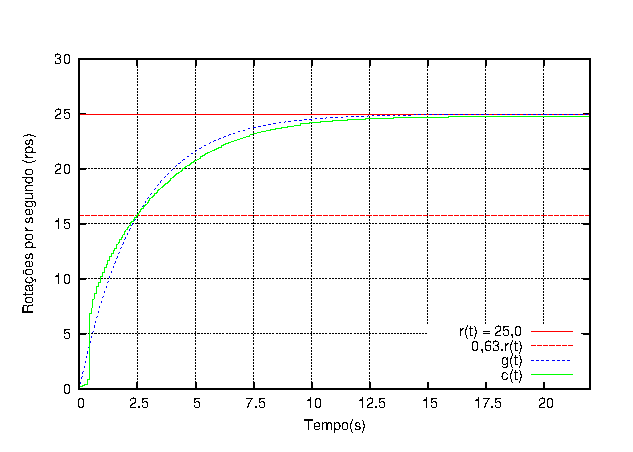
\includegraphics[scale=1]{./imagens/acaoMalhaAbertaTau.eps}
\caption{Ação de Controle em Malha Aberta}
\label{fig:acaoMalhaAberTau}
\end{figure}

A Figura \ref{fig:acaoMalhaAberTau} possui uma linha indicativa que mostra o ponto de intercepção da curva ao valor de 63\% do valor de referência, e empiricamente foi gerado um gráfico com divisões no eixo do Tempo no valor de $\tau = 2,8s $.

Calculando o polo da função:
\begin{equation}
  a = \frac{1}{\tau} = \frac{1}{2,28} = 0,357
\end{equation}

Como $c_{reg} = 25$ e $A$ também é $25$ então na Equação \ref{eq:calcK} $K = a$ e assim temos que:

\begin{equation}
c(t) = \frac{KA}{a}(1-e^{-at}) = \frac{0,357.25}{0,357}(1-e^{-0,357.t}) = 25(1-e^{-0.357.t})
\end{equation}


Aplicando a Transformada de Laplace:

\begin{equation}
  C(s) = \frac{K}{s+a}\frac{A}{s} = \frac{0,357}{s+0,357}\frac{25}{s}
\end{equation}



A finalidade da função de transferência \emph{f(t)} é converter o sinal de referência do tipo \textbf{rps} para seu respectivo parâmetro da modulação por largura de pulso (\textbf{\% PWM}) que aciona o motor.




\subsection{ Duas posições ou Liga-Desliga }
É o tipo de ação de controle mais simples de ser implementado, porém o de menor precisão, pois opera com potência máxima até que o sensor atinja um determinado valor limite, mudando a ação para potência mínima, geralmente zero.

\begin{figure}[!htb]
\center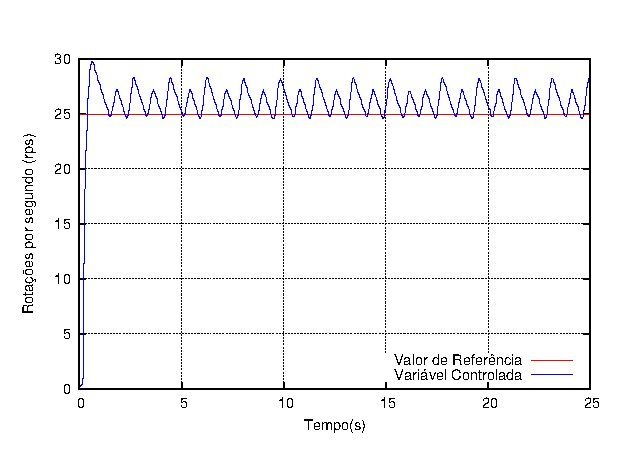
\includegraphics[scale=1]{./imagens/acaoControle-ligaDesliga.eps}
\caption{Ação de Controle Liga-Desliga}
\label{fig:acaoControleLigaDesliga}
\end{figure}

A Figura \ref{fig:acaoControleLigaDesliga} mostra o gráfico obtido no sistema de teste, onde a velocidade de rotação do motor oscila entre os valores de 25 e 30 rps, sendo o valor desejado em 25 rps. 
Todas estas oscilações podem representar perda de energia, pois o motor está recebendo energia em excesso sem necessidade, porém sua implementação é simples e não requer um conhecimento específico e aprofundado de controle.



\begin{figure}[!htb]
\centering
\begin{minipage}{0.8\linewidth}
\begin{lstlisting}
long controlador_LigaDesliga{ long setpoint, long sensor }
{
  if( sensor > setpoint }
    return( 0 );
  else
    return( 100 );
}
\end{lstlisting}
\end{minipage}
\caption{Código da Ação de Controle Liga-Desliga}
\label{fig:codigoAcaoLigaDesliga}
\end{figure}

O código fonte que gerou o resultado obtido na Figura \ref{fig:acaoControleLigaDesliga} é  mostrado na Figura \ref{fig:codigoAcaoLigaDesliga}, sendo apresentada apenas a função que realiza função de controle, que neste caso tem como parâmetros de entrada os valores de \textit{\texttt{setpoint}} e do \textit{\texttt{sensor}} e o seu valor de retorno é o parâmetro de entrada da função de acionamento da modulação por largura de pulso (\textit{PWM - Pulse Width Modulation}), que neste caso utiliza apenas os valores extremos.



\subsection{ Controlador Proporcional (P) } 

 No controle proporcional, o erro é multiplicado por uma constante \emph{kp} gerando o sinal \emph{u{t}}, que é a variável manipulada que atua sobre o sistema \emph{g(t)}.

\begin{equation}
 u(t) = kp . e(t)
\label{eq:acaoP}
\end{equation}


O diagrama de blocos da Figura \ref{fig:malhaFechadaP} mostra o bloco \emph{kp} que tem seu comportamento descrito pela Equação \ref{eq:acaoP} e que atua diretamente sobre o sistema através da variável manipulada $u(t)$.

\begin{figure}[!htb]
\centering
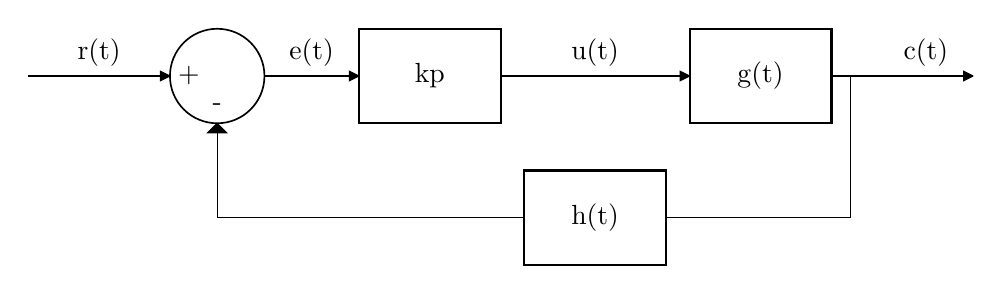
\begin{tikzpicture}[scale=0.6]
%\draw [lightgray](-3,0) grid (17, 2);
%\draw [lightgray](-3,0) grid (17,-3);
%\draw [semithick,red] (0,0) circle (0.1);

\draw (-3,1) -- (0,1);
\draw [fill]( 0,1) -- (-0.2, 1.1) -- ( -0.2,0.9) -- (0,1);
\draw [semithick,black] (1,1) circle (1.0); % Somador
\draw (2.0,1) -- (4,1);
\draw [fill]( 4,1) -- ( 3.8, 1.1) -- ( 3.8,0.9) -- ( 4,1);
\draw [black, thick](4,0) rectangle (7, 2) ; % Controlador 
\draw (7,1) -- (11,1);
\draw [fill]( 11,1) -- (10.8, 1.1) -- (10.8,0.9) -- (11,1);
\draw [black, thick](11,0) rectangle (14, 2) ; % Planta
\draw (14,1) -- (17,1);
\draw [fill](17,1) -- (16.8, 1.1) -- (16.8,0.9) -- (17,1);

\draw [black, thick](7.5,-1) rectangle (10.5, -3) ; % Sensor
\draw (14.4, 1) -- (14.4, -2) -- (10.5,-2);
\draw ( 7.5,-2) -- ( 1, -2) -- (1,0);
\draw [fill](1,0) -- (1.2,-0.2) -- (0.8,-0.2) -- (1,0);

\node [above] at (-1.5,1){r(t)};
\node at (0.4,1){+};
\node at (1,0.4){-};
\node [above] at (3.0,1){e(t)};
\node at ( 5.5, 1){kp};
\node [above] at (9.0,1){u(t)};
\node at (12.5, 1){g(t)};
\node [above] at (16.0,1){c(t)};
\node at ( 9.0,-2){h(t)};

\end{tikzpicture}
\caption{ Diagrama em blocos de sistema de controle em malha fechada utilizando notação matemática}
\label{fig:malhaFechadaP}
\end{figure}

Variando o valor de $kp$ pode-se ver pela Figura \ref{fig:acaoP} que quanto maior o seu valor, mais rápida é a resposta do sistema, ou seja, menor é o tempo necessário para alcançar o valor de referência, porém, depois de um determinado valor, o sistema apresenta um sobressinal, que pode ou não ser tolerável, dependendo das exigências da aplicação.

\begin{figure}[!htb]
\center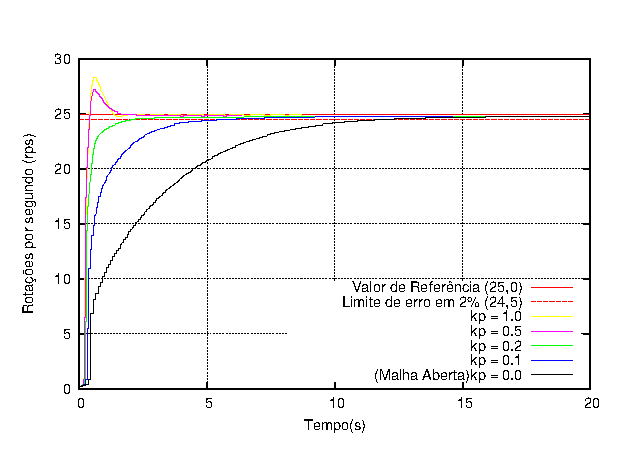
\includegraphics[scale=1.4]{./imagens/acaoP.eps}
\caption{Ação de Controle Proporcional}
\label{fig:acaoP}
\end{figure}

O controlador que foi implementada a função proporcional está apresentado na Figura \ref{fig:codigoControladorP}, onde pode-se verificar a utilização de variáveis do tipo ponto flutuante (\emph{float}) para obtenção de maior precisão nos cálculos e consequantemente, no controle. O nome das variáveis faz alusão a sua representação no diagrama de blocos da Figura \ref{fig:malhaFechadaP}.

A função implementada, declarada na linha 7 possui três parâmetros de entrada e possui um parâmetro de retorno, sendo:
\begin{itemize}
  \item $setpoint$ : recebe o valor de rotação desejado ao sistema, o valor de referência;
  \item $max$ : representa o máximo valor que o sistema alcança;
  \item $sensor$ : recebe o valor de rotação atual da planta;
  \item $return $ : Parâmetro de retorno da função que assume um valor entre 0 e 100, pois é o parâmetro de entrada do controlador PWM que efetua o acionamento do motor.

\end{itemize}



\begin{figure}[!htb]
\centering
\begin{minipage}{0.8\linewidth}
\lstset{firstnumber=1}
\begin{lstlisting}
float kp = 0.1;
float ki = 0.0002;
float kd = 2.0;
float yT, rT, eT, iT, dT, uT;
long  Cout, pwmAlvo;

long controlador{ long setpoint, long max, long sensor }
{
    rT = (float) setpoint;
    yT = (float) sensor;
    pwmAlvo = ((setpoint*100)/max);

    
    eT = rT - yT;
    
    uT = kp*eT;

    Cout = pwmAlvo + uT;

    if( Cout < 0 )
        Cout = 0;
    else if( Cout >= 100 )
        Cout = 100;

    return( Cout );
}
\end{lstlisting}
\end{minipage}
\caption{Código da Ação de Controle Proporcional}
\label{fig:codigoControladorP}
\end{figure}


Nas linhas 9 e 10 os parâmetros de entradas são convertidos em ponto flutuante para realização dos cálculos e atribuidos às respectivas variáveis auxiliares.

A variável \emph{pwmAlvo} recebe o valor percentual da velocidade de referência, como a velocidade mínima é zero, basta dividir o \emph{setpoint} pelo valor \emph{max} e multiplicar por \emph{100} conforme feito na linha 11.


A linha 14 realiza o cálculo do erro, subtraindo do valor de referência (\emph{rT}) o valor do erro (\emph{ht}).

Na linha 18 a variável manipilada recebe o erro (\emph{eT}) sendo multiplicado proporcionalmente pelo coeficiente kp, que caracteriza esta configuração de controle.

A variável \emph{Cout}, é a variável com o valor que será o retorno da função, que serve de parâmetro de entrada ao gerador de sinal PWM que atua sobre o motor.

\emph{Cout} recebe o valor da variável \emph{pwmAlvo} que é a aplicação de um degrau com valor de referência do sistema somado somada a \emph{uT} que possui o valor proporcional ao erro do sistema. 

Inicialmente, considerando o sistema em repouso, o erro possui um valor alto, então, Cout é inicializada com um valor bem maior do que o necessário para gerar o valor de referência, ou seja, um valor de pwm referente a uma velocidade bem maior do que os \emph{25 rps} de referência da aquisição mostrada na Figura \ref{fig:acaoP}. Conforme o sistema começa a girar, e a velocidade aumenta, o erro diminui, o que diminui o incremento ao \emph{pwmAlvo}, até que este incremento seja zero quando o valor lido pelo sensor alcançar o valor de referência, que é o próprio valor do degrau que está em \emph{pwmAlvo}.

O código entre as linhas 20 e 23 são necessárias apenas para não gerar um valor incorreto para o parâmetro do PWM, o que poderia causar falhas no acionamento. 










\subsection{ Controlador Integral (I) }

O controlador integral atua acumulando o erro do sistema, conforme equação descrita abaixo:


\begin{equation}
u(t) = ki \int_{0}^{\infty} e(t) dt
\end{equation}

A resposta apresentada pelo sistema está plotada na Figura \ref{fig:acaoI} e mostra que ao aumentar o valor do coeficiente \emph{ki} o sistema começou a oscilar e demorou mais para estabilizar dentro de um valor limite próximo ao valor de referência. 

\begin{figure}[!h]
\center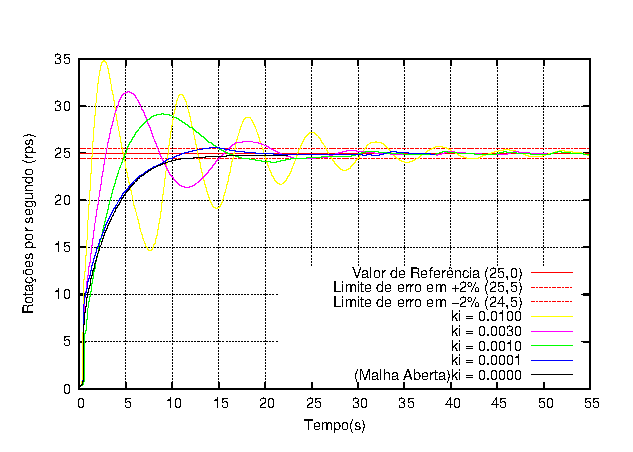
\includegraphics[scale=1.3]{./imagens/acaoI.eps}
\caption{Ação de Controle Integral}
\label{fig:acaoI}
\end{figure}

A Figura \ref{fig:codigoControladorI} mostra o código da função que implementou o controlador com ação integral, responsáveis por gerar propriamente a ação de integração do erro.


\begin{figure}[!htb]
\centering
\begin{minipage}{0.8\linewidth}
\lstset{firstnumber=13}
\begin{lstlisting}

    eT = rT - yT;
    iT += eT * i; 
    uT = iT;
\end{lstlisting}
\end{minipage}
\caption{Código da Ação de Controle Integral}
\label{fig:codigoControladorI}
\end{figure}

A ação de integração é uma somatória de pequenas amostras do erro, que somadas ao longo do tempo levam o sistema a um erro zero, porém demoram mais tempo para alcançar a estabilidade e facilmente geram sobressinal.










\subsection{ Controlador Proporcional + Integral (PI) }

O controlador Proporcional Integral (PI) como o próprio nome indica, é a união das ações de controle que levam seu nome, e busca unir as suas propriedades.
 
\begin{equation}
u(t) = kp.e(t) + ki \int_{0}^{\infty} e(t) dt
\end{equation}

O intuito neste controlador é reduzir o tempo de resposta do sistema pelo controle proporcional e ao mesmo tempo gerar um erro nulo quando a estabilidade é atingida.

\begin{figure}[!htb]
\center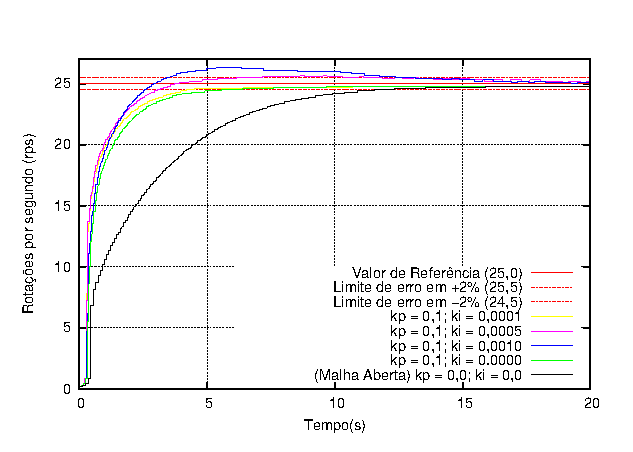
\includegraphics[scale=1.2]{./imagens/acaoPI.eps}
\caption{Ação de Controle Proporcional Integral}
\label{fig:acaoPI}
\end{figure}

Como pode-se ver no gráfico da Figura \ref{fig:acaoPI} foi utilizado um valor de $ki = 0.1$ para obter uma subida em um tempo tido como bom, ou seja, subida mais rápida e sem gerar sobressinal, de acordo com os valores mostrados na Figura \ref{fig:acaoP}.

\begin{figure}[!htb]
\centering
\begin{minipage}{0.8\linewidth}
\lstset{firstnumber=13}
\begin{lstlisting}

    eT = rT - yT;
    iT += eT * i; 
    uT = iT + p*eT;
\end{lstlisting}
\end{minipage}
\caption{Código da Ação de Controle Proporcional Integral}
\label{fig:codigoControladorPI}
\end{figure}

O código da Figura \ref{fig:codigoControladorPI} mostra a implementação das funções de controle proporcional e integral, sendo que a linha 15 mostra a somatória característica do controle integral.










\subsection{ Controlador Proporcional + Derivativo (PD) }

A ação de controle proporcional e derivativo propicia uma resposta mais rápida, pois a ação derivativa gera um grande erro se houver variações abruptas.

\begin{equation}
u(t) = kp.e(t) + kd. \frac{d e(t)}{dt}
\end{equation}

A figura \ref{fig:acaoPD} mostra que a resposta do sistema é a mais rápida dos ações de controle estudadas, e também gera o maior sobressinal. 


\begin{figure}[!htb]
\center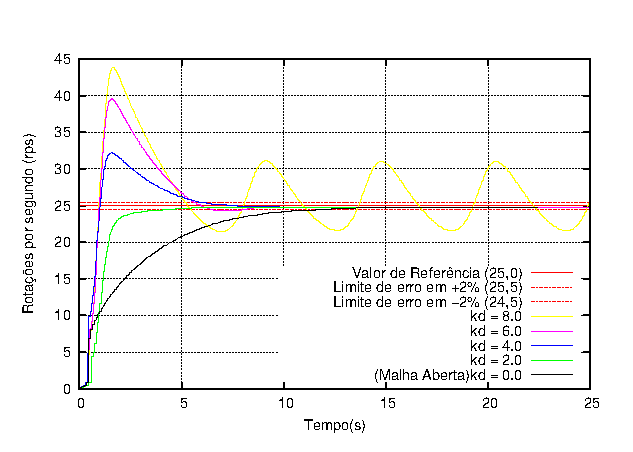
\includegraphics[scale=1.1]{./imagens/acaoPD.eps}
\caption{Ação de Controle Proporcional Derivativo}
\label{fig:acaoPD}
\end{figure}

 A linha 13 da Figura \ref{fig:codigoControladorPD} mostra como foi codificada a ação de controle Derivativa modificada.

\begin{figure}[!htb]
\centering
\begin{minipage}{0.8\linewidth}
\lstset{firstnumber=13}
\begin{lstlisting}
    dT = (eT - (rT-yT)) * d;
    eT = rT - yT;

    uT = dT + p*eT;
\end{lstlisting}
\end{minipage}
\caption{Código da Ação de Controle Proporcional Derivativo}
\label{fig:codigoControladorPD}
\end{figure}

A ação de controle derivativa (PD) é modificada pois é utilizada a diferença do erro na iteração anterior com o erro com os dados atuais, diferente do que ocorre com o controlador PD teórico, onde a derivada implica na diferença entre o valor atual e uma pequena variação positiva do tempo, ou seja, uma amostra futura, que é impossível de ser obtida na pratica. 










\subsection{ Controlador Proporcional + Integral + Derivativo (PID) }

O controlador Proporcional Integral Derivativo é uma das configurações mais utilizadas por sua versatilidade, unindo as características que permitem ajustar o tempo de subida, o sobressinal e o erro de estado estacionário, conforme a necessidade e a aplicação.

\begin{equation}
u(t) = kp.e(t) + ki \int_{0}^{\infty} e(t) dt + kd. \frac{d e(t)}{dt}
\end{equation}

O controlador PID pode ser implementado de diversas formas, pode ter o parâmetro proporcional influenciando diretamente as demais ações, ou não, como neste caso onde as ações de controle são utilizadas de forma independentes, e o erro é utilizado para cada uma das partes da soma do sinal da variável manipulada ($u(t)$).

\begin{figure}[!htb]
\center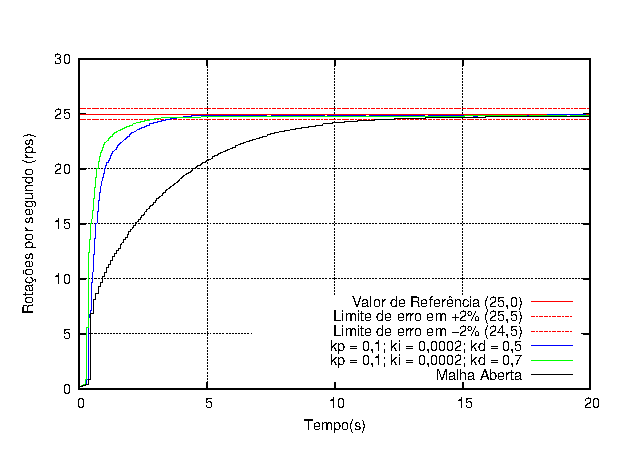
\includegraphics[scale=1.4]{./imagens/acaoPID.eps}
\caption{Ação de Controle Proporcional Integral Derivativo}
\label{fig:acaoPID}
\end{figure}

Os dois sinais utilizando o controle PID utilizou parâmetros já testados nos controladores anteriores para obter um resultado desejado, onde o sistema responde de forma bem rápida ao estímulo de entrada, tendo um tempo de subida entre 3 e 4 segundos para atingir a estabilidade com erro de estado estacionário menor do que 2\%, sem gerar sobressinal.


Em comparação ao sinal de controle em malha aberta, que a estabilidade é alcançada em um tempo de aproximadamente 12 segundos, o ganho de velocidade é consideravel para o sistema estudado, pois foi reduzido a pelo menos um terço do tempo original.

A Figura \ref{fig:codigoControladorPID} mostra a codificação completa dos parâmetros do PID, onde pode-se perceber que sua implementação é simples, apesar da teoria ser complexa. 

\begin{figure}[!htb]
\centering
\begin{minipage}{0.8\linewidth}
\lstset{firstnumber=13}
\begin{lstlisting}
    dT = (eT - (rT-yT)) * d;
    eT = rT - yT;
    iT += eT * i; 
    uT = p*eT + iT + dT;
\end{lstlisting}
\end{minipage}
\caption{Código da Ação de Controle Proporcional Integral Derivativo}
\label{fig:codigoControladorPID}
\end{figure}


Para o microcontrolador efetuar as subtrações é algo que requer pouco processamento, mas as multiplicações são bem mais complexas e exigem mais memória e tempo de processamento, e é claro que trabalhando em ponto flutuante esta complexidade também é muito grande. O controlador utilizado possui uma unidade de processamento de ponto flutuante, o que possibilitou uma performance capaz de efetuar todos os cálculos sem afetar a leitura de velocidade do sistema.


%%%%%%%%%%%%%%%%%%%%%%%%%%%%%%%%%%%%%%%%%%%%%%%%%%%%%%%%%%%
\section{Requisitos de desempenho do sistema}
%%%%%%%%%%%%%%%%%%%%%%%%%%%%%%%%%%%%%%%%%%%%%%%%%%%%%%%%%%%

Os sistemas de controle buscam atender os chamados requisitos de desempenho do sistema, que de um modo geral se efetuam através de modificações das características da relação entrada/saída para se obter os valores desejados dessa relação, ou ainda ajustar o comportamento da saída para uma dada entrada específica.

Os principais e mais comuns requisitos de desempenho dos sistemas são associados a velocidade de resposta, presença ou não de oscilações e a exatidão da resposta do sistema em relação ao valor desejado, chamada de erro de regime estacionário.

O erro de regime estacionário, mostrada na Figura \ref{fig:funcaoResposta}, é uma medida que vai tender a zero em sistemas ideais, mas que na realidade não alcança o valor zero, assim assume-se um valor aceitável, 5\% do valor da resposta desejada para sistemas não críticos e 2\% para sistemas de maior grau de criticidade, para assumir que o sistema entrou em estabilidade, e a resposta real é aceita como tendo atingido o valor de resposta desejada. 

\begin{figure}[!htb]
\center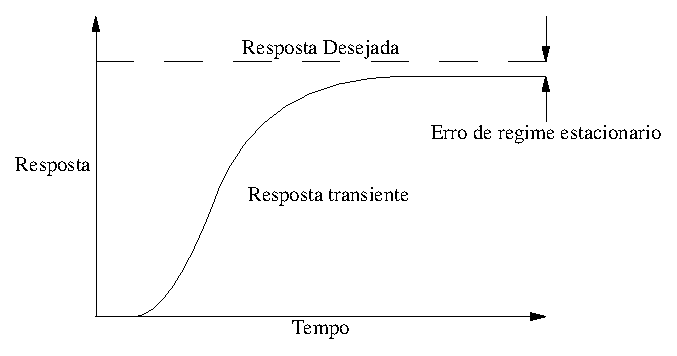
\includegraphics[scale=1]{./pic/C400grafico.eps}
\caption{Gráfico da função Resposta}
\label{fig:funcaoResposta}
\end{figure}

Para realizar o controle de um sistema é necessário que estejam bem definidos os seus requisitos, que são os objetivos a serem atendidos. Quando um sistema por si só já atende aos requisitos, não há a necessidade de controle. De forma oposta, é projetado o sistema de controle, que pode ser em malha aberta ou fechada, clássico ou moderno dependendo das características físicas do sistema. 

Para a execução de um sistema de controle podem ser verificados requisitos do sistema de duas formas básicas, sendo a primeira através dos testes e levantamento empírico da sua curva de resposta ou através de seu modelo matemático, quando trabalha-se com elementos já bem estudados e com a equação que representa seu comportamento empírico bem estabelecida por diversos estudos anteriores.



\newpage



%%%%%%%%%%%%%%%%%%%%%%%%%%%%%%%%%%%%%%%%%%%%%%%%%%%%%%%%%%%
\section{Controle Moderno Não Convencional \\ Lógica Paraconsistente}
%%%%%%%%%%%%%%%%%%%%%%%%%%%%%%%%%%%%%%%%%%%%%%%%%%%%%%%%%%%

O controle moderno trata de sistemas multivariáveis, não lineares ou variantes no tempo de forma mais apropriada do que o controle clássico, reduzindo a complexidade das expressões para que haja a possibilidade de um processamento satisfatório.
Dentro do universo do controle moderno, existe ainda o controle convencional que utiliza a análise de sistemas de controle no espaço de estados, que utiliza n-equações de primeira ordem combinadas em uma equação diferencial vetor-matricial, de forma a simplificar e possibilitar o trabalho com uma quantidade de variáveis alta sem que haja um grande impacto no processamento.  \cite{Ogata} 
Outra forma de controle moderno é denominada controle não convencional, aonde estão situadas diversas técnicas como controle adaptativo, algoritmos adaptativo e genético, redes neurais, as lógicas Fuzzy e Paraconsistente, que é alvo da abordagem do presente trabalho, entre outras.

A lógica, como ramo filosófico que trata das relações de coerência racional e discursiva, proposições e conclusões, tem como origem a Grécia Antiga com o seu primeiro arranjo formal em \emph{Tópicos} de Aristóteles por volta de 340 a.C. Apesar de suas bases serem conhecidas e discutidas por diversos pensadores anteriores, não havia a formalização de uma teoria bem fundada, apenas o tratamento de ideias como consistência e consequências da contraditoriedade por exemplo. 

Os princípios da lógica enunciadas por Aristóteles são basilares para a teoria clássica e moldaram o pensamento e a noção de consistência, ou não contraditoriedade, estreitamente conectadas ao conceito de completude e podem ser descritos formalmente assim:


\begin{enumerate}
\item Princípio de Identidade: 
    \begin{math}
	A \rightarrow B 
	\textrm{ ou } 
	\forall x(x=x);
    \end{math}

\item Princípio do Terceiro Excluído:
    \begin{math}
	A \vee \neg A
	\textrm{ ou }
	\forall x(Ax \vee \neg Ax);
    \end{math}

\item Princípio da Não Contradição: 
    \begin{math}
	\neg (A \wedge \neg A)
	\textrm{ ou }
	\forall x\neg(Ax \wedge \neg Ax).
    \end{math}

\end{enumerate}

O grande desenvolvimento da lógica, principalmente nos séculos XIX e XX, forneceu ferramental para caracterização e tratamento preciso da lógica clássica e também possibilitou o desenvolvimento de sistemas lógicos não clássicos, possibilitando rearranjos, experimentações e questionamentos de dogmas secularmente estabelecidos.

Uma questão que já havia sido objeto de estudo por diversos pensadores desde os pré-socráticos, como Heráclito e sua doutrina da harmonia dos opostos, é a questão da contradição, que por vezes incomodou-os mas que nunca havia sofrido um tratamento formal como o desenvolvido por Newton C. A. da Costa(1929- ) e Stanislaw Jaskiwski(1906-1965), que propuseram e desenvolveram sistemas lógicos que fossem capazes de lidar com essas inconsistências. 

Para (da Costa e Marconi, 1989), ao restringir em um certo sistema lógico o princípio da não contradição, obtém-se um resultado que pertence à lógica denominada Paraconsistente.


Assim sendo, para uma dada teoria, se houver um símbolo de negação, como por exemplo "\emph{$\neg $}", se em qualquer fórmula fechada \emph{A} não for demonstrável \emph{$A$} e \emph{$\neg A $} a teoria é consistente (não contraditória), senão, ela é inconsistente(contraditória).


Teoria é definida por (Evandro Luís Gomes, 2013 p.4) como sendo:
\citacao
{
...um conjunto de fórmulas(expressões bem formuladas) de uma linguagem, fechadas por uma determinada relação de consequência, que caracteriza a lógica subjacente à teoria, da qual ela herda todas as suas características estruturais como, por exemplo, consistência(não contraditoriedade) e completude.
}

Na lógica clássica, uma teoria é completa, se e somente se, for consistente para toda a fórmula fechada \emph{A} onde \emph{A} e \emph{$\neg A$} é teorema da teoria e a teoria é trivial ou supercompleta se todas as fórmulas expressáveis forem demonstráveis, tanto \emph{A} quanto \emph{$ \neg A$}.


Sendo que toda a lógica paraconsistente, não se pode deduzir qualquer fórmula à partir de uma fórmula \emph{A} e sua negação \emph{$\neg A$}, mostrando assim que as noções de inconsistência (contraditoriedade) e trivialidade são de fato independentes.



%A lógica paraconsistente, segundo (Evandro Luis Gomes, 2013) 
%"Apesa do problema da existência de contradições aceitáveis já vir chamando a atenção de lógicos e filósofos pelo menos desde o tempo de Aristóteles, até o aparecimento das lógicas paraconsistentes não se dispunha de um aparato lógico para o estudo das contradiçẽos." 
%Arruda(1990, p.5-6) in Evandro Luis Gomes, 2013 p.5

%"E, como da Costa mesmo reconhecera antes, em 1958, a não trivialidade é que é decisiva ao exercício teórico-racional."
%Evandro Luis Gomes, 2013 p.439



%%%%%%%%%%%%%%%%%%%%%%%%%%%%%%%%%%%%%%%%%%%%%%%%%%%%%%%%%%%%
\subsection{Reticulado de Hasse}
%%%%%%%%%%%%%%%%%%%%%%%%%%%%%%%%%%%%%%%%%%%%%%%%%%%%%%%%%%%%

A lógica paraconsistente sendo apropriada para tratar dados inconsistentes foi utilizada em 1987, por H. Blair e V. S. Subrahmanian para representar e codificar o funcionamento de bancos de dados inconsistentes. Pouco depois Costa, Subrahmanian e Vago propuseram a lógica paraconsistente anotada e sua extensão a uma lógica de predicados paraconsistente anotada de primeira ordem. 

Nas lógicas paraconsistentes anotadas, uma proposição $P$ utiliza um reticulado formado por pares ordenados tal que: 

\begin{center}
\begin{equation}
\tau = \{ ( \mu , \lambda ) \mid \mu ,\lambda \in [0,1] \subset \Re \}
\end{equation}
\end{center}

de acordo com graus de cresça das constantes anotacionais do reticulado de Hasse, associado à Lógica Paraconsistente Anotada com anotação de dois valores (LPA2v), formalmente descritas como 

\begin{center}
\begin{equation}
  \tau = \{ \top , V, F, \bot \}
\end{equation}
\end{center}

os quais descrevem os extremos do reticulado como sendo inconsistente, verdadeiro, falso e paracompleto, respectivamente. 

\begin{figure}[!htb]
\center\includegraphics{./pic/C421reticuladoHasse.eps}
\caption{Reticulado finito de Hasse}
\label{fig:reticuladoHasse}
\end{figure}

Para toda proposição $P$ há um par de valores, chamada de anotação, $(\mu , \lambda )$, onde $\mu$ é o grau de evidência favorável e $\lambda $ é o grau de evidência desfavorável, representada como  $P_{( \mu , \lambda )}$ .

%$P_{( \mu , \lambda )}$
Como exemplificação, para uma proposição $P \equiv$ \emph{"A temperatura do aquecedor atingiu o valor desejado."}, assume-se dois especialistas para realizarem a leitura dos valores da anotação. Em um sistema físico, os especialistas geralmente são sensores, como neste caso, poderiam ser sensores de temperatura.

\begin{itemize}
\item 
$\mu$ = grau de evidência favorável (especialista 1), ou seja, com quanto de certeza, em um intervalo fechado $[0,1]$, sendo 0 para grau nulo de certeza e 1 grau máximo de certeza para a dada proposição $P$;

\item
$\lambda$ = grau de evidência desfavorável (especialista 2), ou seja, com quanto de certeza, em um intervalo fechado $[0,1]$, sendo 0 o grau nulo de certeza à evidência desfavorável e 1 o grau máximo de certeza à evidência desfavorável para a dada proposição $P$.

\end{itemize}


Assim, podemos interpretar da seguinte forma os valores da anotação para as posições extremas do reticulado finito de Hasse:

\begin{itemize}
\item 
$(\mu, \lambda ) = (1,0)$ : Há um grau de evidência favorável total e um grau de evidencia desfavorável nulo, ou seja, a afirmação da proposição é máxima e sua negação é nula, assim,  $P$ é \emph{Verdadeira} e \emph{A temperatura do aquecedor atingiu o valor desejado};

\item 
$(\mu, \lambda ) = (0,1)$ : Há um grau de evidência favorável nulo e um grau de evidencia desfavorável máximo, ou seja, a afirmação da proposição é nula e sua negação é máxima, assim,  $P$ é \emph{Falsa} e \emph{A temperatura do aquecedor não atingiu o valor desejado};

\item 
$(\mu, \lambda ) = (1,1)$ : Há um grau de evidência favorável máximo e também um grau de evidencia desfavorável máximo, ou seja, a afirmação da proposição é máxima e sua negação também é máxima, assim,  $P$ é \emph{Inconsistente} e \emph{A temperatura do aquecedor atingiu e não atigiu o valor desejado}, contradição;

\item 
$(\mu, \lambda ) = (0,0)$ : Há um grau de evidência favorável nulo e também um grau de evidencia desfavorável nulo, ou seja, a afirmação da proposição é nula e sua negação também é nula, assim,  $P$ é \emph{Indeterminada} e \emph{A temperatura do aquecedor nem atingiu o valor desejado e nem não atingiu o valor desejado}, situação paracompleta.

\end{itemize}

Os graus de evidência podem assumir valores não extremos:

\begin{itemize}
\item 
$(\mu, \lambda ) = (0.8,0.3)$ : Crê-se com grau de evidência favorável de 80\% e um grau de evidencia desfavorável de 30\%  que \emph{A temperatura do aquecedor atingiu do valor desejado}.
\end{itemize}

Existe um operador de negação ($\sim $) sobre $\tau$ de forma que :
\begin{center}
\begin{equation}
\sim  : \mid \tau \mid \rightarrow \mid \tau , \sim(\mu, \lambda ) = (\lambda, \mu )
\end{equation}
\end{center}

Então,
\begin{center}
\begin{equation}
P_{(0.8,0.3)} \leftrightarrow \textrm{"   "} \sim P_{(0.3,0.8)}
\end{equation}
\end{center}

\begin{itemize}
\item 
$(\mu, \lambda ) = (0.8,0.3) = \sim (0.3,0.8)$ : Não crê-se que há um grau de evidência favorável de 30\% e um grau de evidencia desfavorável de 80\% que \emph{A temperatura do aquecedor atingiu do valor desejado}.
\end{itemize}



%%%%%%%%%%%%%%%%%%%%%%%%%%%%%%%%%%%%%%%%%%%%%%%%%%%%%%%%%%%%
\subsection{Quadrado Unitário no Plano Cartesiano - QUPC}
%%%%%%%%%%%%%%%%%%%%%%%%%%%%%%%%%%%%%%%%%%%%%%%%%%%%%%%%%%%%

Uma outra forma de representação da anotação é utilizando o Quadrado Unitário no Plano Cartesiano (QUPC) no qual são transpostos os pontos extremos às respectivas posições de acordo com o par ordenado,  $(\mu, \lambda ) \leftrightarrow (x,y) $, assim o eixo $x$ corresponde ao grau de evidência favorável e o eixo $y$ corresponde ao grau de evidência desfavorável, conforme mostrado na Figura \ref{fig:reticuladoQUPC}.



\begin{figure}[!htb]
\center\includegraphics{./pic/C422qupc.eps}
\caption{Representação do reticulado no quadrado unitário no plano cartesiano}
\label{fig:reticuladoQUPC}
\end{figure}

Os pontos extremos assim representam:

\begin{itemize}
\item $A: (0,0) = \bot \Rightarrow $ Paracompleto;
\item $B: (0,1) = F \Rightarrow $ Falso;
\item $C: (1,1) = \top \Rightarrow $ Contradição;
\item $D: (1,0) = V \Rightarrow $ Verdade.
\end{itemize}

O segmento de reta $\overline{BD}$, entre os pontos referentes às condições $Verdade$ e $Falso$, conforme mostrado na Figura \ref{fig:retaPerfeitamenteDefinida}, é denominada de \emph{Reta Perfeitamente Definida} e dada uma anotação $(\mu, \lambda )$ situada nela, a soma das evidências anotadas é sempre o valor unitário do quadro. 

\begin{figure}[!htb]
\center\includegraphics{./pic/C424retaPerfeitamenteDefinida.eps}
\caption{Representação da Reta Perfeitamente Definida}
\label{fig:retaPerfeitamenteDefinida}
\end{figure}

A relação dos graus de evidência da anotação quando coincidente à Reta Perfeitamente Definida é: 

\begin{center}
\begin{equation}
\mu + \lambda = 1
\label{eq:evidenciaUnitaria1}
\end{equation}
\end{center}

Assim, temos que:

\begin{center}
\begin{equation}
\mu + \lambda - 1 = 0
\label{eq:evidenciaUnitaria}
\end{equation}
\end{center}


Os graus de evidência não precisam apresentar valores complementares, possuem independência entre si, assim das Equações  
\ref{eq:evidenciaUnitaria1} e 
\ref{eq:evidenciaUnitaria} 
é elaborado o conceito de 
\emph{Grau de Contradição}($G_{ct}$), 
assim temos: 

\begin{center}
\begin{equation}
G _{ct} = \mu + \lambda - 1
\label{eq:grauIncerteza}
\end{equation}
\end{center}

quanto mais próximo da Reta Perfeitamente Definida, menor o grau de contradição apresentado pelos graus de evidência. 
Quanto mais afastado da Reta Perfeitamente Definida estiver o ponto, e mais próximo aos pontos A ou C, maior é o grau de contradição. 

Quando a anotação estiver situada na região entre os pontos BCD, acima da reta perfeitamente definida, o grau de contradição é denominado 
\emph{Grau de Inconsistência} ($G_{it}$), 
e isso ocorre quando, $\mu \ge \lambda $, de forma oposta, quando $\mu < \lambda $ a anotação está situada na região entre os pontos BAD, abaixo da reta perfeitamente definida, e o grau de contradição é denominado 
\emph{Grau de Indefinição} ($G_{id}$), 
então pode-se dizer que:

\begin{center}
\begin{equation}
-1 \le G _{id}  <  0 \le G _{it} \le 1
\label{eq:grauInconsistenciaIndefinicao}
\end{equation}
\end{center}
e
\begin{center}
\begin{equation}
-1 \le G _{ct} \le 1
\label{eq:grauInconsistenciaIndefinicao1}
\end{equation}
\end{center}


O segmento de reta $\overline{ AC }$ , entre os pontos referentes às condições \emph{Paracompleto} e \emph{Contradição}, conforme mostrado na Figura \ref{fig:retaPerfeitamenteIndefinida}, é denominada de \emph{Reta Perfeitamente Indefinida} e dada uma anotação $(\mu, \lambda )$ situada nela, a subtração das evidências anotadas é sempre zero, $\mu = \lambda$, e de forma contrária, quando a anotação está posicionada de forma não coincidente à Reta Perfeitamente Indeterminada, significa que $\mu \neq \lambda$.

\begin{figure}[!htb]
\center\includegraphics{./pic/C426retaPerfeitamenteIndefinida.eps}
\caption{Representação da Reta Perfeitamente Indefinida}
\label{fig:retaPerfeitamenteIndefinida}
\end{figure}

A relação dos graus de evidência para uma anotação cuja posição coincide com a Reta Perfeitamente Indefinida é: 

\begin{center}
\begin{equation}
\mu - \lambda = 0
\label{eq:evidenciaIndefinida}
\end{equation}
\end{center}

De forma análoga ao Grau de contradição, da Equação \ref{eq:evidenciaIndefinida} é elaborado o conceito de \emph{Grau de Certeza} ($G _c$), assim temos que: 

\begin{center}
\begin{equation}
G _{c} = \mu - \lambda
\label{eq:grauCerteza}
\end{equation}
\end{center}

Quando os graus de evidência, favorável e desfavorável, são iguais, não há certeza em relação à proposição, mas quando são diferentes, alguma certeza pode ser inferida, até a condição máxima onde uma das evidências é total (1) e a outra é nula (0), caracterizando a condição verdadeira ou falsa, afastando o ponto anotado da Reta Perfeitamente Indefinida. 

Quando a anotação situa-se entre os pontos ABC do QUPC, o grau de certeza é denominado \emph{Grau de Falsidade ($G _f$)}, e tal condição ocorre quando $\mu < \lambda $, caso contrário, se $\mu \ge \lambda $, a anotação situa-se entre os pontos ACD do QUPC, e o grau de certeza é denominado \emph{Grau de Verdade ($G _v)$}, então pode-se dizer que:

\begin{center}
\begin{equation}
-1 \le G _{f}  <  0 \le G _{v} \le 1
\label{eq:grauVerdadeFalsidade}
\end{equation}
\end{center}
e
\begin{center}
\begin{equation}
-1 \le G _{c} \le 1
\label{eq:grauCertezaIntervalo}
\end{equation}
\end{center}


Graficamente são representadas como mostra a Figura \ref{fig:retasgcgct}:

\begin{figure}[!htb]
\center\includegraphics{./pic/C428retasgcgct.eps}
\caption{Representação dos Graus de Certeza e Contradição em um plano cartesiano}
\label{fig:retasgcgct}
\end{figure}

A representação ainda é dividia em algumas partes, dependendo da aplicação, estabelecendo quais são os limites que definem cada estado, Verdadeiro, Falso, Paracompleto, Contradição e outros mais que forem pertinentes à aplicação, estão representados pelas linhas tracejadas na Figura \ref{fig:valorControle} e são definidos como:

\begin{itemize}
\item \emph{V $_{scc}$ : Valor limite superior de Controle de Certeza};
\item \emph{V $_{icc}$ : Valor limite inferior de Controle de Certeza};
\item \emph{V $_{sci}$ : Valor limite superior de Controle de Incerteza};
\item \emph{V $_{sci}$ : Valor limite inferior de Controle de Incerteza}.

\end{itemize}

\begin{figure}[!htb]
\center\includegraphics{./pic/C429valorControle.eps}
\caption{Representação dos valores de controle}
\label{fig:valorControle}
\end{figure}

Uma divisão em 12 partes é mostrada na Figura \ref{fig:reticuladoLPA2v} com seus respectivos estados intermediários definidos conforme \cite{JoaoInacio}, sendo 4 regiões extremas:


\begin{figure}[!htb]
\center\includegraphics{./pic/C430gcgct.eps}
\caption{Representação do reticulado da LPA2v subdividido em 12 regiões}
\label{fig:reticuladoLPA2v}
\end{figure}


\begin{itemize}
\item V : Verdadeiro;
\item F : Falso;
\item $\top$ : Contradição;
\item $\bot$ : Paracompleto.
\end{itemize}
e 8 regiões intermediárias: 
\begin{itemize}
\item Qv $\rightarrow  \top$ : Quase Verdade tendendo à Contradição;
\item Qv $\rightarrow  \bot$ : Quase Verdade tendendo à  Paracompleto;
\item Qf $\rightarrow  \top$ : Quase Falso tendendo à Contradição;
\item Qf $\rightarrow  \bot$ : Quase Falso tendendo à Paracompleto;
\item $\top \rightarrow $ f : Contradição tendendo à Falso;
\item $\top \rightarrow $ v : Contradição tendendo à Verdadeiro;
\item $\bot \rightarrow $ f : Paracompleto tendendo à Falso;
\item $\bot \rightarrow $ v : Paracompleto tendendo à Verdadeiro.

\end{itemize}

O reticulado subdividido em 12 regiões como mostrado, é aplicado em situações nas quais a tomada de decisão utiliza estados discretos bem definidos para atuação, onde para cada posição da anotação e respectivamente um estado do reticulado, uma ação é tomada, assim sendo, a quantidade de subdivisões está fortemente dependente da aplicação.



%%%%%%%%%%%%%%%%%%%%%%%%%%%%%%%%%%%%%%%%%%%%%%%%%%%%%%%%%%%%
\subsection{A LPA2v aplicada em Controle}
%%%%%%%%%%%%%%%%%%%%%%%%%%%%%%%%%%%%%%%%%%%%%%%%%%%%%%%%%%%%

A LPA2v aplicada em sistemas de controle utiliza além dos conceitos já estabelecidos, duas outras definições para sua implementação e são elas o \emph{ Grau de Certeza Real ($G _{CR}$)} e o \emph{Grau de Evidência Real ($\mu _{ER}$)} além de trabalhar alguns conceitos básicos de geometria, e pelo fato de possuir uma resolução simples do ponto de vista matemático, motiva este trabalho pela sua implementação eficaz com relação ao controle clássico que exige uma matemática elaborada, dificultando sua implementação em dispositivos de baixo custo e que não possuem hardware específico de processamento de sinais. 


Para a implementação do sistema de controle paraconsistente, primeiramente é necessário que seja definida a proposição que será a base para as análises e tomadas de decisões.

\begin{center}
$ P \equiv $ 
\emph{"A temperatura do aquecedor atingiu o valor desejado."}
\end{center}

Para trabalhar com essa proposição são necessárias pelo menos duas variáveis, sendo uma delas com o valor de temperatura desejada e outra com o valor atual de temperatura. Essas duas variáveis são representadas por meio de duas anotações, mas que antes precisam ser normalizadas. 

\textbf{Variável 1:} 
Valor desejado ou Set point = 37 $^{\circ}$C. 

\begin{equation}
( \mu _{d}, \lambda _{d} ) = (1,0)
\label{eq:setpoint}
\end{equation}

Sendo:

$\mu _{d}$ : grau de evidência favorável ao valor desejado. 

$\lambda _{d}$ : grau de evidência desfavorável ao valor desejado.

Quando o aquecedor atingir a temperatura de 37 $^{\circ}$C, 
crê-se com grau de evidência favorável máxima e grau de evidência desfavorável mínima que a proposição \emph{P} é verdadeira, como mostrado na Equação \ref{eq:setpoint}.



\textbf{Variável 2:} 
Valor de temperatura atual lido pelo sensor: 20 $^{\circ}$C no início do processo.

Supondo, hipoteticamente para facilitar o entendimento, um sensor com range de operação entre 0 e 100 $^{\circ}$C que será lido, linearmente no intervalo de 0 a 10V e normalizado para o intervalo fechado [0,1]. Assim são calculados os graus de evidência:

\begin{equation}
\mu _{a} = 
\frac{Ta - Tmin}{Td - Tmin}
\label{eq:miatual}
\end{equation}

Sendo:

$\mu _{a}$ : Grau de evidência favorável para a leitura da temperatura atual;

\emph{Ta :} Temperatura atual lida pelo sensor;

\emph{Tmin :} Temperatura mínima de leitura pelo sensor de temperatura. Nesse caso, 0 $^{\circ}$C;

\emph{Td :} Temperatura desejada que o aquecedor alcance, estabelecida em 37 $^{\circ}$C.

A normalização pode ser realizada diretamente, desde que todas as variáves da Equação \ref{eq:miatual} estejam na mesma grandeza e na mesma escala, assim os graus de evidência não apresentam dimensão.

Substituindo as variáveis em \ref{eq:miatual}:

\begin{equation}
\mu _{a} = 
\frac{20 - 0}{37 - 0} = 0,54
\label{eq:miatualnumeros}
\end{equation}

Para o valor de $\mu _{a}$ da Equação \ref{eq:miatualnumeros} podemos afirmar que \emph{crê-se com grau de evidência favorável que foi atingido 54\% do percurso para a proposição ser verdadeira.} Como se pode ver, a temperatura inicial proposta foi de 20$^{\circ}$C que é pouco mais da metade da temperatura desejada de 37$^{\circ}$C, caso seja alterada a temperatura desejada para 50$^{\circ}$C, o valor de $\mu _{d}$ seria de 0,4, ou seja, a variável atual seria 40 \% do valor desejado. 

Calculando o grau de evidência desfavorável:

\begin{equation}
\lambda _{a}= 1 - \mu _{a}
\label{eq:lambdaatual}
\end{equation}

Substituindo as variáveis:

\begin{equation}
\lambda _{a}= 1 - 0,54 = 0,46
\label{eq:lambdaatualnumeros}
\end{equation}

O que resulta em uma anotação para a leitura de temperatura atual de: 

\begin{equation}
( \mu _{a}, \lambda _{a} ) = (0,54 , 0,46)
\label{eq:valoratual}
\end{equation}

Calcula-se então o Grau de Contradição (Equação \ref{eq:grauIncerteza} ) e o Grau de Certeza (Equação \ref{eq:grauCerteza}) cruzando os dados das anotações da seguinte forma:

\begin{equation}
G _{ct} = \mu _{d} + \lambda _{a} - 1
\label{eq:grauContradicaoCruzado}
\end{equation}

\begin{equation}
G _{c} = \mu _{d} - \lambda _{a}
\label{eq:grauCertezaCruzado}
\end{equation}


Substituindo (\ref{eq:miatualnumeros}) e (\ref{eq:lambdaatualnumeros}) em (\ref{eq:grauContradicaoCruzado}):

\begin{equation}
G _{ct} = 1 + 0,46 - 1 = 0,46
\label{eq:grauContradicaoResulta}
\end{equation}

Substituindo (\ref{eq:miatualnumeros}) e (\ref{eq:lambdaatualnumeros}) em (\ref{eq:grauCertezaCruzado}):

\begin{equation}
G _{c} = 1 - 0,46 = 0,54
\label{eq:grauCertezaResulta}
\end{equation}

Graficamente pode ser representado como na Figura \ref{fig:gcgctExemplo}.

\begin{figure}[!htb]
\center\includegraphics{./pic/C440gcgctExemplo.eps}
\caption{Representação de Gc = 0.54 e Gct = 0.46}
\label{fig:gcgctExemplo}
\end{figure}



%%%%%%%%%%%%%%%%%%%%%%%%%%%%%%%%%%%%%%%%%%%%%%%%%%%%%%%%%%%%
%%%%%%%%%%%%%%%%%%%%%%%%%%%%%%%%%%%%%%%%%%%%%%%%%%%%%%%%%%%%

